Map\footnote{
    W. Hirsch, S. Smale, Introduction to Chaos.
} $f$ is \textbf{chaotic}, if \\
\begin{itemize}
    \item Periodic points are dense everywhere in $\vc{E}$.
    \item Orbits are mixed (almost): \\
    let $U_1$, $U_2$ $\subset \vc{E}$. $ \forall x_0 \in U_1 \; \exists N \in \mathbb{N}: f^N (x_0) \in U_2. $ 
    \item $f$ Sensitive to the i. c. \\
    $\forall x_0 \in \vc{E}, \; \forall U_{\varepsilon}(x_0) \; \exists y_0 \in U_{\varepsilon}, \exists N\in \mathbb{N} \colon |f^n(x_0) - f^n(y_0)| > \beta.$  
\end{itemize}

\begin{figure}[h]
    \centering
    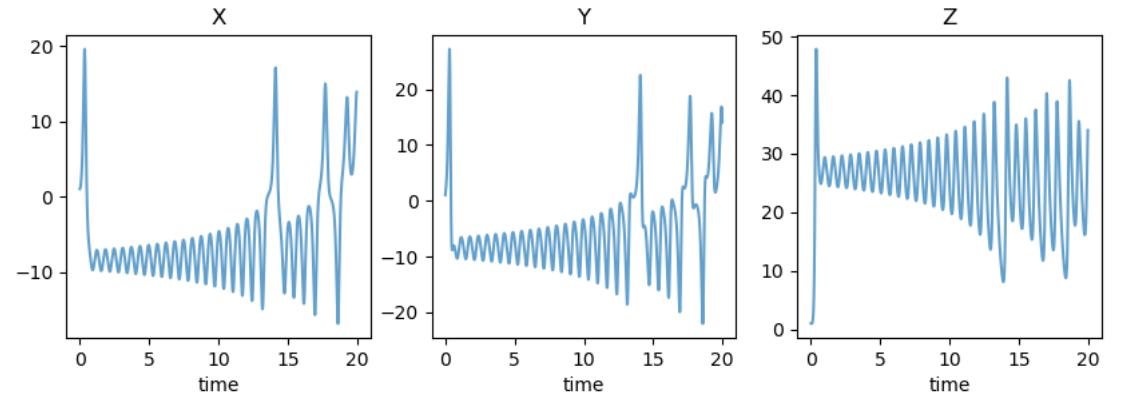
\includegraphics[width=0.55\textwidth]{images/xyz.png}
    \hspace{5 mm}
    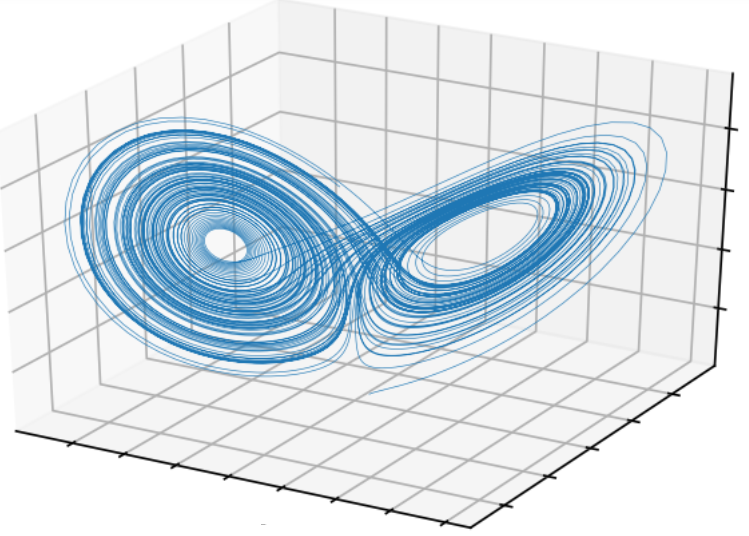
\includegraphics[width=0.35\textwidth]{images/attr_L.png}
    %\caption{}
    %\label{fig:}
\end{figure}
